Reactive functions are functions that can read reactive values and call other reactive functions. Whenever a reactive value changes, any reactive functions that depended on it are marked as "invalid" and will be automatically re-executed if necessary. If a reactive function is marked as invalid, all other reactive functions that have called it recently will also be marked as invalid. In this way, invalidations are propagated by functions that depend on each other.
\begin{figure}[h]
\centering % para centralizarmos a figura
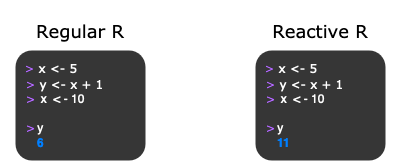
\includegraphics[width=7cm]{images/react.png} 

\caption{Example of Regular R - Reactive R}
\label{figura:qualquernome}
\end{figure}

In our application we use reactive functions as it is a way to control which parts of the application are updated, avoiding unnecessary calculations that can make your application slow.